\documentclass[a4paper, 11pt]{article}
%%%
%%% Loading Packages
\usepackage[utf8]{inputenc}
\usepackage[english]{babel}
\usepackage{natbib}
\bibliographystyle{apj}
\bibliographystyle{abbrvnat}
\usepackage{comment} % enables the use of multi-line comments (\ifx \fi) 
\usepackage{lipsum} %This package just generates Lorem Ipsum filler text. 
\usepackage{fullpage} % changes the margin
\usepackage[utf8]{inputenc}
\usepackage[table]{xcolor}
\usepackage{tabularx}
\usepackage{color}
\usepackage{float}
\usepackage{pdfpages}
\usepackage{etoolbox}
\usepackage{pdfpages}
% \usepackage[backref]{hyperref}
\usepackage{hyperref}
\usepackage[all]{hypcap}
\hypersetup{
    colorlinks=true,
    citecolor=blue,
    % linkcolor=blue,
    filecolor=magenta,      
    urlcolor=cyan,
}

\newcommand{\kmsMpc}{\mbox{$\textrm{km}\ \textrm{s}^{-1}\ \textrm{Mpc}^{-1}$}}
\newcommand{\rband}{\textit{r}-band }
\newcommand{\gband}{\textit{g}-band }
\defcitealias{Cacciato2009}{C09}

%%%%%%%%%%%%%%%%%%%%%%%%%%%%%%%%%%%%%%%%%%%%%%%%%%%%%%%%%%%%%%%%%%%%%%%%%%%%%%%
%%
%% Definitions
% \renewcommand*{\backref}[1]{[#1]}
\urlstyle{same}

%% If-statements
\newtoggle{paper}
\toggletrue{paper}
% \togglefalse{paper}

%%
%%
%%%%%%%%%%%%%%%%%%%%%%%%%%%%%%%%%%%%%%%%%%%%%%%%%%%%%%%%%%%%%%%%%%%%%%%%%%%%%%%
\begin{document}

%%
%% Header
\noindent
\large \today \hfill \textbf{Victor Francisco Calderon} \\
\normalsize . \hfill Ph.D. Candidate\\
\normalsize . \hfill Adviser: \href{http://astro.phy.vanderbilt.edu/~berlinaa/}{Prof. Andreas Berlind}\\
\normalsize . \hfill \href{https://as.vanderbilt.edu/astronomy/}{Department of Physics \& Astronomy} \\
\normalsize . \hfill \href{http://www.vanderbilt.edu/}{Vanderbilt University} \
\normalsize\hfill  \\


%%%%%%%%%%%%%%%%%%%%%%%%%%%%%%%%%%%%%%%%%%%%%%%%%%%%%%%%%%%%%%%%%%%%%%%%%%%%%%%
%%%
%%% Project Proposal
\begin{centering}
\section*{ECO, Resolve A, and Resolve B Catalogues}\label{sec:catalogues}
\end{centering}

\section{Mock Catalogues}\label{sec:mock_catls}

We construct a set of mock catalogues from a cosmological 180 
$h^{-1} \mathrm{Mpc}$ N-body cube
simulation that traces the evolution of dark matter in the Universe.
The dark matter (DM) halos are found by applying a Friends-of-Friends
algorithm \citep[FoF;]{Davis1985a} to link together particles 
separated by a specified linking length equal to 0.2 times the 
mean inter-particle separation of the DM particles. The total mass of the 
dark matter halo is the sum of all the contributing DM particles. The 
suite assumes \textit{Planck 2015} \citep{Planck2016} cosmology and uses 
the \citet{Warren2006} halo mass function.
$\Omega_{m,0} = 0.307$,
$\Omega_{b,0} = 0.0486$,
$\Omega_{\Lambda,0} = 0.6918$,
$h = H_{0}/$ (100 \kmsMpc) = 0.7,
mass function.

We use an HOD \citep{Berlind2002} model to populate the DM halos
with galaxies. We differentiate between central and satellite 
gaalxies in the halo, each following different probability distributions.
For each set of mock catalogues, the numbers of central and satellite
galaxies as a funciton of halo mass were chosen to reproduce 
the number density, $n_{gal}$ of the ECO survey. The central galaxy is 
located at the minimum of the potential well of the halo, and is 
assigned the mean velocity of the DM halo. Satellite galaxies 
are assigned the positions and velocities of randomly chosen DM particles 
bound to the host halo.

%%%% CLF for Luminosities
\subsection{Conditional Luminosity Function}\label{sub:clf}
To assign luminosities to the mock galaxies, we adopt the formalism of the 
\textit{conditional luminosity function} $\Phi (L|M)$ 
\citep[CLF;][]{Yang2003, VanDenBosch2003} and 
\cite[\citetalias{Cacciato2009};][]{Cacciato2009}, which 
gives the number of galaxies with luminosities in the range of 
$L \pm dL/2$ that are member of a halo of mass $M$. This allows us to 
create a link between the distribution of DM halos and that of the 
residing galaxies, while also differentiating between central and 
satellite galaxies (c.f. Eq. 32-39 in \citetalias{Cacciato2009}).

For the purpose of the project, we want to mimic the luminosity function of 
ECO. We assign real ECO \rband absolute magnitudes taken from the 
ECO survey. We make use of the ranking of luminosities from the 
CLF method and use it to determine the order, in which galaxies get 
assigned absolute magnitudes. We determine the ratio of the number 
of mock galaxies to the number of real galaxies, i.e. $f_{mr}$.
We assign the most luminous ECO \rband absolute magnitude to the 
first $f_{mr}$ most luminous mock galaxies, according to the CLF. We 
keep assigning the next most luminous SDSS \rband absolute magnitde 
to the next set of $f_{mr}$ most luminous mock galaxies, until all 
mock galaxies have been assigned an SDSS \rband magnitude. This method 
will then preserve the \rband luminosity function in the data.

%%% Extra Properties
\subsection{Other galaxy properties}\label{sub:other_prop}
We want to assign other properties, other than \rband absolute magnitudes, 
to the mock galaxies. For each mock galaxy, we find the galaxy in the data 
that has the closest \rband absolute magnitude to that of the mock galaxy.
Then we assign all the associated galaxy properties of the \textit{real} 
galaxy to the mock galaxy. In that way, we are assigning real galaxy property 
values to the mock galaxies.

%% Geometrical and Redshift cuts
\subsection{Geometrical and Redshift Cuts}\label{sub:geo_cuts}
As the final step, we construct volume-limited galaxy galaxy redshift 
survey catalogues from the simulation box. Depending on the survey geometry, 
we place a virtual observer at different positions in the box, in order 
to maximize the total number of mock catalogues out from the box. We first 
place a virtual observer at the starting position in the box, and define 
right ascension (RA) and declination (Dec) for each galaxy with respect 
to the virtual observer. Then, for every mock galaxy, we compute the 
angular coordinates and rdshift, including the effect due to the line-of-sight 
peculiar velocity of the galaxy, i.e. \textit{redshift-space distortions}.
After carving out the geometry of the survey and only selecting those 
mock galaxies that fall within the survey geometrical limits, we 
place the virtual observer to the next location, and repeat the same procedure.
The final result is a set of volume-limtied galaxy is a set of volume-limited 
galaxy galaxies in redshift-space, with the exact same geometry as 
ECO, Resolve A, or Resolve B. We construct set of 59, 104, and 8 volume-limited 
mock galaxy catalogues for Resolve A, Resolve B, and ECO surveys, respectively.
The resulting mock catalogues can be downloaded from Section~\ref{sec:download}.

%% Group Finder
\subsection{Group-Finding algorithm and Group Catalogue}\label{sec:alg_sec}
Additionally, we want to assign galaxies to galaxy groups. We use the 
\citet{Berlind2006} FoF algorithm with a set of linking lengths 
$l_{\perp} = 0.07$ and $l_{\parallel} = 1.1$, in units of the mean 
inter-galaxy separation. For each group, we calculate the properties shown 
in the \textit{README.md} file attached.

\section{Survey of Volumes}\label{sec:volumes}

The volumes used to create the catalogues are the following (in units of 
$h^{-3}\textrm{Mpc}^{3}$  ):\\[10pt]

\begin{centering}
% \begin{table}[h]
\begin{tabular}{|c|c|r|}
\hline
Survey    & Number of Mocks & Volume [$h^{-3}\textrm{Mpc}^{3}$] \\\hline
Resolve A & 59              & 20,957.7789388\\ \hline
Resolve B & 104             & 15,908.063125\\ \hline
ECO       & 8               & 192,294.221932 \\\hline
\end{tabular}
% \caption{Details about the different surveys.}
% \end{table}

\end{centering}

\section{Download Mock Catalogues}\label{sec:download}

You can download the mock catalogues for the 3 different survey at:

\begin{itemize}
    \item ECO: \href{http://vpac00.phy.vanderbilt.edu/~caldervf/ECO_A_B_Updated/ECO}{Link}
    \item Resolve A: \href{http://vpac00.phy.vanderbilt.edu/~caldervf/ECO_A_B_Updated/Resolve_A}{Link}
    \item Resolve B: \href{http://vpac00.phy.vanderbilt.edu/~caldervf/ECO_A_B_Updated/Resolve_B/}{Link}
    \item Mass Function: \href{http://vpac00.phy.vanderbilt.edu/~caldervf/ECO_A_B_Updated/Mass_Function/}{Link}
\end{itemize}

%%%% README
\section{README}\label{sec:README}
% Attach PDF
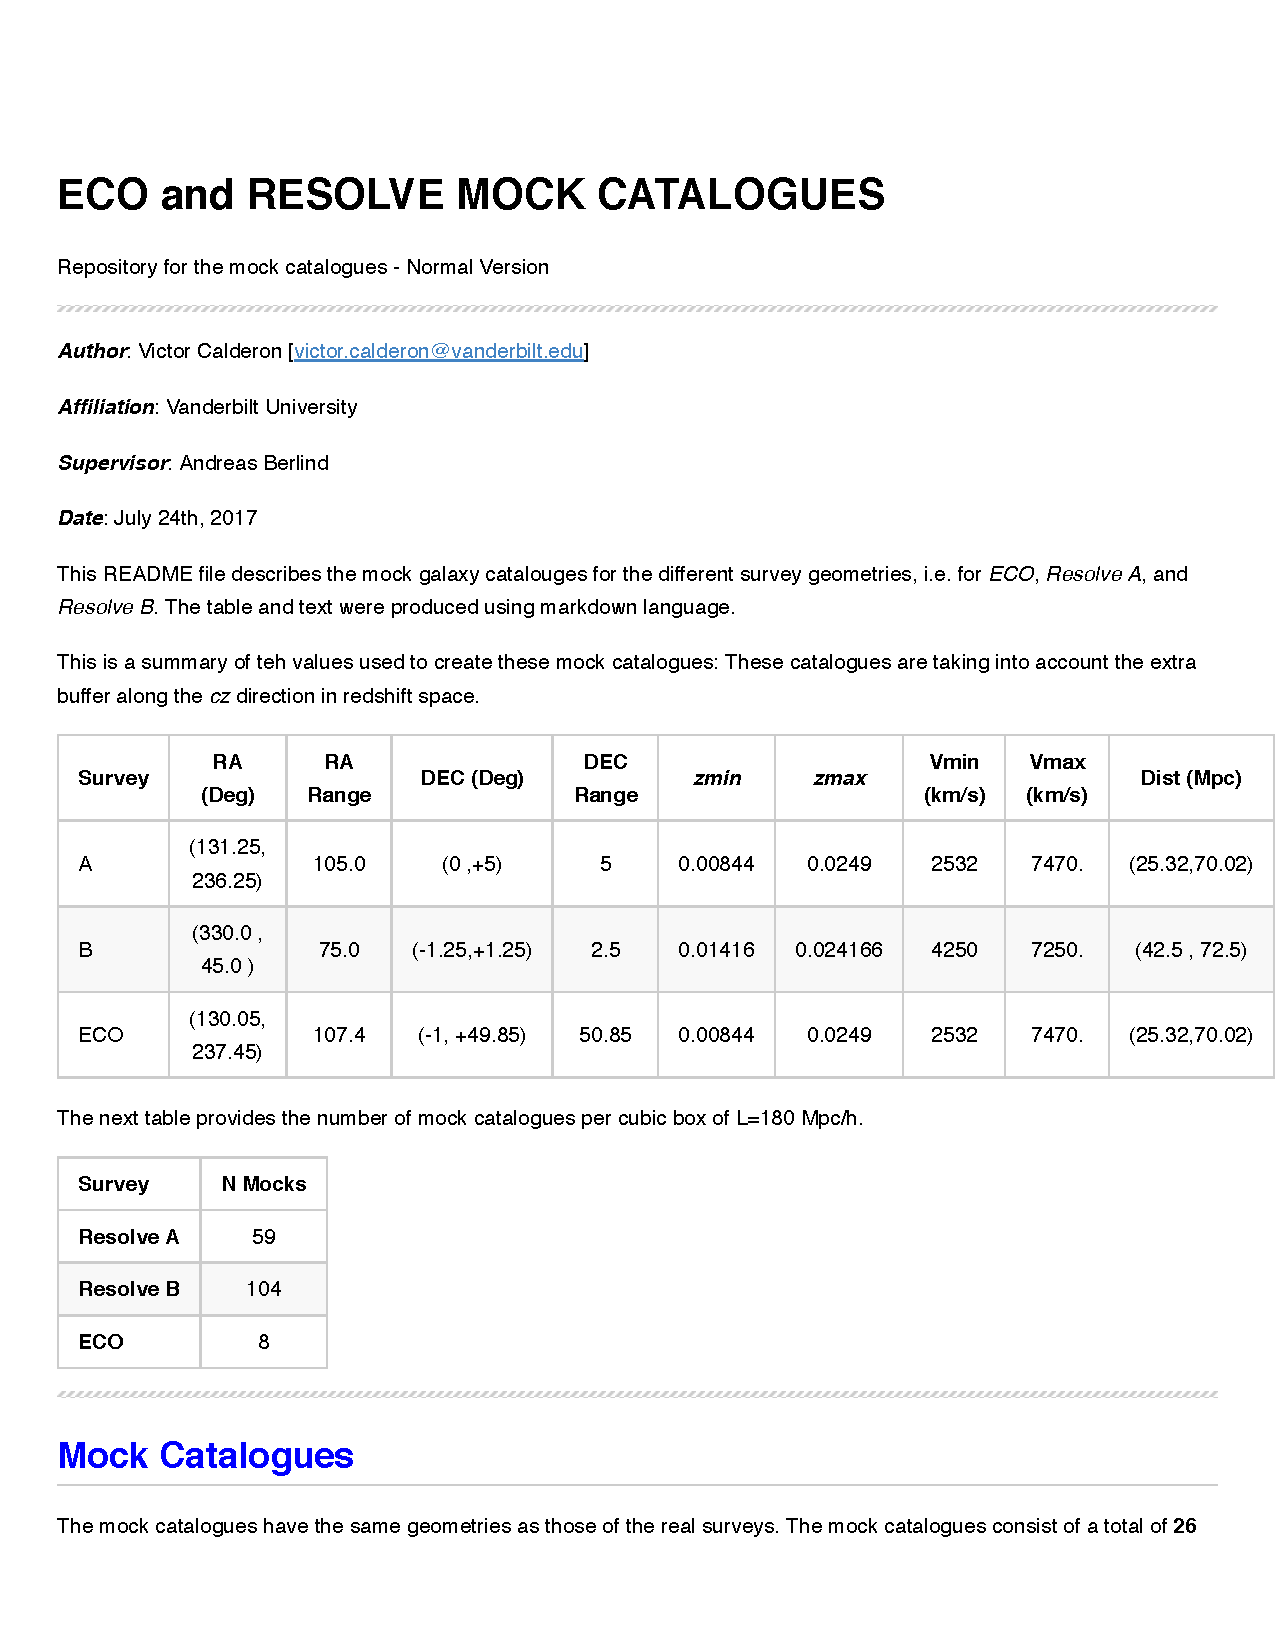
\includepdf[scale=.9, pages={1-4}]{./README.pdf}


%% Bibliography
\bibliography{VC_Publications}

\end{document}
